\chapter{Introducción específica} % Main chapter title

\label{Chapter2}

%----------------------------------------------------------------------------------------
%	SECTION 1
%----------------------------------------------------------------------------------------
En el presente capítulo se brinda una introducción a diferentes tecnologías utilizadas en el trabajo y una explicación del funcionamiento general del sistema implementado. Se presentan además los requerimientos y la planificación del trabajo.

\section{Bluetooth}

La tecnología Bluetooth opera en la banda de frecuencia industrial, científica y médica (ISM) sin licencia de 2.4GHz. Admite múltiples opciones de radio que permiten a los desarrolladores desarrollar productos que cumplen con requisitos de conectividad específicos de cada aplicación. 

Ya sea que un producto transmita audio de alta calidad entre un teléfono inteligente y un altavoz, transfiera datos entre una tableta y un dispositivo médico, o envíe mensajes entre miles de nodos en una aplicación de automatización de edificios, las tecnologías Bluetooth Low Energy (LE) y Basic Rate/Enhanced Data Rate (BR/EDR) están diseñadas para satisfacer las distintas necesidades de los desarrolladores de todo el mundo \cite{bluetooth}.


\subsection{Bluetooth Low Energy (LE)}

La tecnología Bluetooth Low Energy (LE) está diseñada para funcionar con muy baja potencia. Permite un funcionamiento confiable en la banda de frecuencia de 2.4 GHz, ya que aprovecha un sólido enfoque de espectro ensanchado por salto de frecuencia que transmite datos a través de 40 canales \cite{bluetooth}.

Esta tecnología, brinda a los desarrolladores una enorme flexibilidad, incluidas múltiples opciones en la capa física (PHY) que admiten velocidades de datos de 125 Kb/s a 2 Mb/s, múltiples niveles de potencia, entre 1 mW y 100 mW, así como múltiples opciones de seguridad \cite{bluetooth}. 

Bluetooth LE también admite múltiples topologías de red, incluidas redes punto a punto, de broadcast y de malla.


\subsection{Bluetooth clásico}

La tecnología Bluetooth clásica, también conocida como Bluetooth Basic Rate/Enhanced Data Rate (BR/EDR), está diseñada para un funcionamiento de baja potencia y también aprovecha un sólido enfoque de salto de frecuencia adaptable, que transmite datos en 79 canales \cite{bluetooth}.

Esta tecnología incluye múltiples opciones en la capa física (PHY) que admiten velocidades de datos de 1 Mb/s a 3 Mb/s, múltiples niveles de potencia, entre 1 mW y 100 mW, múltiples opciones de seguridad y una topología de red punto a punto \cite{bluetooth}.

\subsection{Comparación de tecnologías Bluetooth}

El Bluetooth clásico y el Bluetooth LE tienen, en principio, fines muy diferentes \cite{bluetoothV}.

\begin{itemize}

\item El Bluetooth clásico puede manejar muchos datos, pero consume mucha más energía.

\item El Bluetooth LE se utiliza para aplicaciones que no necesitan intercambiar grandes cantidades de datos, y por lo tanto puede funcionar con la energía de una batería durante años a un menor costo.

\end{itemize}

Todo depende de lo que se desee conseguir. En general, el Bluetooth clásico se utiliza principalmente en dispositivos de audio inalámbricos, como conexiones telefónicas, auriculares y altavoces inalámbricos.

El Bluetooth LE es más frecuente en dispositivos utilizados como prendas de vestir (wearables), tales como smartwatches o sensores de frecuencia cardíaca, en dispositivos inteligentes del IoT, como termómetros o alarmas y en accesorios que funcionan con pilas, como un teclado inalámbrico de ordenador.

Es importante notar que las versiones de Bluetooth a partir del estándar 4.0, en adelante, cuentan tanto con Bluetooth clásico, como con Bluetooth LE. Por tanto, a partir de esta versión los dispositivos pueden configurarse para que funcionen de acuerdo con uno de los dos estándares.

La tabla \ref{tab:Bluetooth} muestra una comparación de las principales características de ambas tecnologías Bluetooth: LE y BR/EDR.

\begin{table}[h]
	\centering
	\caption[Tecnologías Bluetooth]{Tabla comparativa de tecnologías Bluetooth.}
	\begin{tabular}{l c c}    
		\toprule
		\textbf{} 	 & \textbf{Bluetooth low energy (LE)} & \textbf{Bluetooth clásico}\\
		\midrule
		\begin{tabular}[c]{@{}l@{}}Bandas de \\ frecuencia\end{tabular}          & \begin{tabular}[c]{@{}l@{}}Banda ISM de 2.4GHz \\ (2.402 - 2.480 GHz utilizados)\end{tabular}                                                     & \begin{tabular}[c]{@{}l@{}}Banda ISM de 2.4GHz\\ (2.402 - 2.480 GHz utilizados)\end{tabular}                          \\
Canales                                                                  & \begin{tabular}[c]{@{}l@{}}40 canales con espaciado de 2 \\ MHz (3 canales publicitarios, \\ 37 canales de datos)\end{tabular}                    & \begin{tabular}[c]{@{}l@{}}79 canales con espaciado de \\ 1 MHz\end{tabular}                                          \\
\begin{tabular}[c]{@{}l@{}}Uso de los \\ canales\end{tabular}            & \begin{tabular}[c]{@{}l@{}}Espectro ensanchado por \\ salto de frecuencia (FHSS)\end{tabular}                                                     & \begin{tabular}[c]{@{}l@{}}Espectro ensanchado por \\ salto de frecuencia (FHSS)\end{tabular}                         \\
Modulación                                                               & GFSK                                                                                                                                              & GFSK, $\pi$/4 DQPSK, 8DPSK                                                                                                \\
\begin{tabular}[c]{@{}l@{}}Consumo de\\ energía\end{tabular}             & \begin{tabular}[c]{@{}l@{}}$\sim$0.01x 0.5x de referencia\\ (dependiendo del caso de uso)\end{tabular}                                            & 1 (valor de referencia)                                                                                               \\
\begin{tabular}[c]{@{}l@{}}Velocidad de\\ datos\end{tabular}             & \begin{tabular}[c]{@{}l@{}}LE 2M PHY: 2 Mb/s\\ LE 1M PHY: 1 Mb/s\\ LE Coded PHY (S=2): 500 Kb/s\\ LE Coded PHY (S=8): 125 Kb/s\end{tabular}       & \begin{tabular}[c]{@{}l@{}}EDR PHY (8DPSK): 3 Mb/s\\ EDR PHY ($\pi$/4 DQPSK): 2 Mb/s\\ BR PHY (GFSK): 1 Mb/s\end{tabular} \\
\begin{tabular}[c]{@{}l@{}}Potencia máxima\\ de Transmision\end{tabular} & \begin{tabular}[c]{@{}l@{}}Clase 1: 100 mW (+20 dBm)\\ Clase 1.5: 10 mW (+10 dbm)\\ Clase 2: 2.5 mW (+4 dBm)\\ Clase 3: 1 mW (0 dBm)\end{tabular} & \begin{tabular}[c]{@{}l@{}}Clase 1: 100 mW (+20 dBm)\\ Clase 2: 2.5 mW (+4 dBm)\\ Clase 3: 1 mW (0 dBm)\end{tabular}  \\
\begin{tabular}[c]{@{}l@{}}Topologias\\ de red\end{tabular}              & \begin{tabular}[c]{@{}l@{}}Punto a punto (incluida piconet)\\ Transmisión\\ Malla\end{tabular}                                                    & Punto a punto (incluida piconet)\\
		\bottomrule
		\hline
	\end{tabular}
	\label{tab:Bluetooth}
\end{table}

%----------------------------------------------------------------------------------------

\section{Sistema propuesto}

La figura \ref{fig:DiagramaBloques} muestra un diagrama de bloques del sistema propuesto donde se puede apreciar que es completamente inalámbrico, ya que el dispositivo llamador se conecta a la terminal de sala a través de Bluetooth. Esto permite eliminar la limitación de conectar solo dos dispositivos llamadores, además de eliminar los riesgos asociados al cableado. También lo hace más cómodo y versátil, pues el paciente podrá llevarlo a donde sea que vaya y lo podrá utilizar sin estar necesariamente en la cama. Por ejemplo si necesita ir al baño y estando ahí requiere ayuda, no necesita volver a la cama para solicitar atención.

\begin{figure}[htpb]
	\centering
	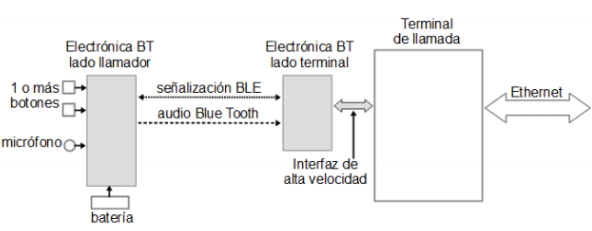
\includegraphics[scale=0.5]{./Figures/DiagramaDeBloques.png}
	\caption{Diagrama en bloques del sistema propuesto.}
	\label{fig:DiagramaBloques}
\end{figure}

El sistema que se desarrolla en este trabajo agrega la electrónica tanto del lado del llamador como del lado de la terminal, cuyo dispositivo Bluetooth acepta varios llamadores Bluetooth, que le envían novedades. La terminal de sala  a su vez redirecciona las novedades de cada paciente a la terminal de llamada.

El terminal de llamada, como ya hacía el anterior sistema, notifica vía Ethernet a la enfermera, y en caso de ser necesario establece una llamada entre el paciente y la enfermera.

%----------------------------------------------------------------------------------------

\section{Requerimientos}

Los requerimientos del nuevo sistema de llamado a enfermera son:

\begin{enumerate}

\item Al pulsar uno de los botones del dispositivo llamador, la terminal de sala deberá iniciar una llamada con una terminal de enfermería.

\item Una vez que la terminal de enfermería conteste a la llamada de la terminal de sala, o cuando la terminal de enfermería realice una solicitud de iniciar una llamada, la terminal de sala indicará al dispositivo llamador, que corresponda, encender su micrófono e iniciar el envío de la señal de audio.

\item Cada dispositivo llamador debe poder identificarse con un ID único de manera que pueda ser registrado en una terminal de sala.

\item La terminal de sala deberá registrar los IDs de los llamadores correspondientes a las camas que tenga en el cuarto, y no deberá aceptar conexiones de otros llamadores.

\item La transmisión de audio debe realizarse por Bluetooth LE.

\item La transmisión de audio debe realizarse utilizando el codec g711 ulaw empleado en el software actual.

\item El dispositivo llamador debe permanecer en modo de bajo consumo mientras no esté en una llamada, o el paciente presione un botón.

\item La terminal de sala además de sus tareas habituales debe estar a la escucha de los mensajes de los dispositivos llamadores que tenga registrados.

\item Al requerimiento de la terminal de enfermería, la terminal de sala debe poder determinar a qué dispositivo llamador dirigir la solicitud.

\item El software debe permitir modificar sus parámetros operativos y almacenarlos en memoria segura.

\item El software no debe alterar las condiciones de operación actuales  del sistema.

\item Se deberá diseñar dos placas eléctricas, una para el módulo de expansión a conectarse a la terminal de sala, y otra para el dispositivo llamador.

\end{enumerate}

Los requerimientos del  modulo de expansión para la terminal son:

\begin{enumerate}

\item Conectar de 1 a 3 dispositivos llamadores.

\item Notificar a la terminal de sala las solicitudes del paciente para que inicie una llamada con la terminal de enfermería.

\item Notificar a la terminal de sala cuando un dispositivo llamador se encuentre con baja batería.

\item Al estar en llamada, el módulo de expansión deberá ignorar las peticiones de otros llamadores y solo retransmitir la señal de audio a la terminal de sala.

\end{enumerate}

Los requerimientos del dispositivo llamador son:

\begin{enumerate}

\item Medir el nivel de batería del dispositivo y notificar al módulo de expansión de la terminal de sala al que se encuentre conectado.

\item Notificar a la terminal de sala sobre las solicitudes del paciente según el botón presionado.

\item Leer señal de audio y transmitirla a la terminal de sala cuando se encuentre en llamada.

\end{enumerate}

\section{Planificación}

En la figura \ref{fig:ActivityOnNode} se presenta la planificación inicial aprobada para el desarrollo del presente proyecto donde se aprecia el camino crítico para su ejecución, habiéndose estimado un total de 615 horas de trabajo.

\begin{figure}[htpb]
	\centering
	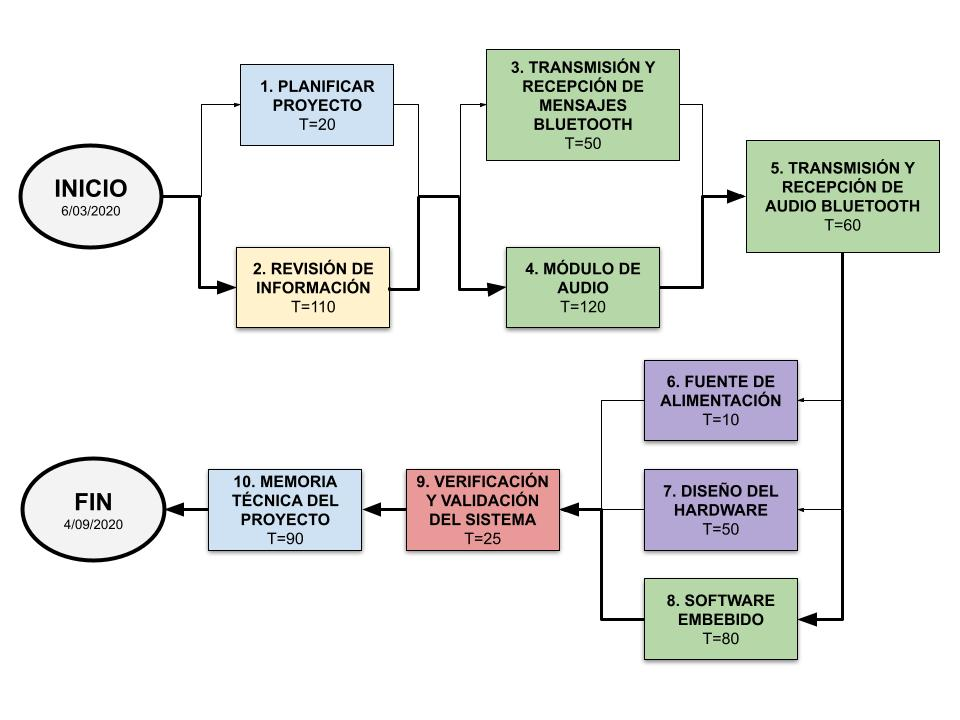
\includegraphics[scale=0.4]{./Figures/ActivityOnNode.jpg}
	\caption{Diagrama activity on node del trabajo.}
	\label{fig:ActivityOnNode}
\end{figure}

Esta planificación inicial no se cumplió de acuerdo a lo previsto debido a que algunos supuestos del proyecto no se cumplieron, entre los que se destacan:

\begin{itemize}

\item El tiempo requerido para el desarrollo del software resultó mayor al previsto. Además de ello, se tuvo un retraso en el inicio de esta actividad ya que debido a la cuarentena que se decretó de un momento a otro, no se dispuso oportunamente del material necesario para desarrollar el proyecto.

\item Hubo dificultad al conseguir algunos componentes electrónicos necesarios, particularmente, el micrófono para poder hacer pruebas durante el desarrollo.

\item El tiempo requerido para el desarrollo del hardware resultó mayor al previsto. La empresa cuenta con un fabricante de placas de su confianza, que se encuentra en China, y debido a la coyuntura originada por la aparición del COVID-19 se han tenido dificultades en la comunicación y transporte.

\end{itemize}

No obstante, si bien los plazos fueron más largos de lo previsto, el trabajo pudo realizarse en forma exitosa, como se muestra en los siguientes capítulos.